
\begin{frame}{\citetitle{MarcoNuno_Revista_2021_10_00}$^*$  (1)}

\begin{columns}
\begin{column}{0.70\textwidth}
	\begin{itemize}
		\item Se propone un protitipo para monitorear de manera remota temperatura y humedad
        \item Aplicaciones particulares: cultivos (tradicionales, invernaderos, sistemas hidropónicos o acuapónicos, etc)
		\item El sensor estan enviando información utilizando el protocolo MQTT y un servidor especializado (Broker)
        \item Se implementó una aplicación móvil que muestra notificaciones y estadísticas del comportamiento de dichas variables
	\end{itemize}
\end{column}
\begin{column}{0.30\textwidth}  
\begin{center}
     \begin{tabular}{cc}
         \includegraphics[width=0.98\textwidth]{2021_IoT_JoseRamon/figs/Figura_Refrigeradores.jpg}\\         
      \end{tabular}
\end{center}
\end{column} 
\end{columns} 


%\footnotetext[1]{\fullcite{MarcoNuno_ReporteTecnico2022_C}}
%\setcounter{footnote}{0}
\footfullcite*{MarcoNuno_Revista_2021_10_00}
\end{frame}



\begin{frame}{\citetitle{MarcoNuno_Revista_2021_10_00} (2)}
\begin{columns}
\begin{column}{0.40\textwidth}
Componentes hardware:
\begin{itemize}
    \item Tarjeta Nodemcu Esp8266 WiFi. 
    \item Sensor de Humedad/Temperatura DHT22, alimentado por el NodeMCU, con una mayor precisón en comparación con su predesor el DTH22
    \item Router para conectividad remota a internet
	\end{itemize}
\end{column}
\begin{column}{0.60\textwidth}  
\begin{center}
     \begin{tabular}{c}
\includegraphics[width=0.48\textwidth]{2021_IoT_JoseRamon/figs/resultadodelsensor.jpg}
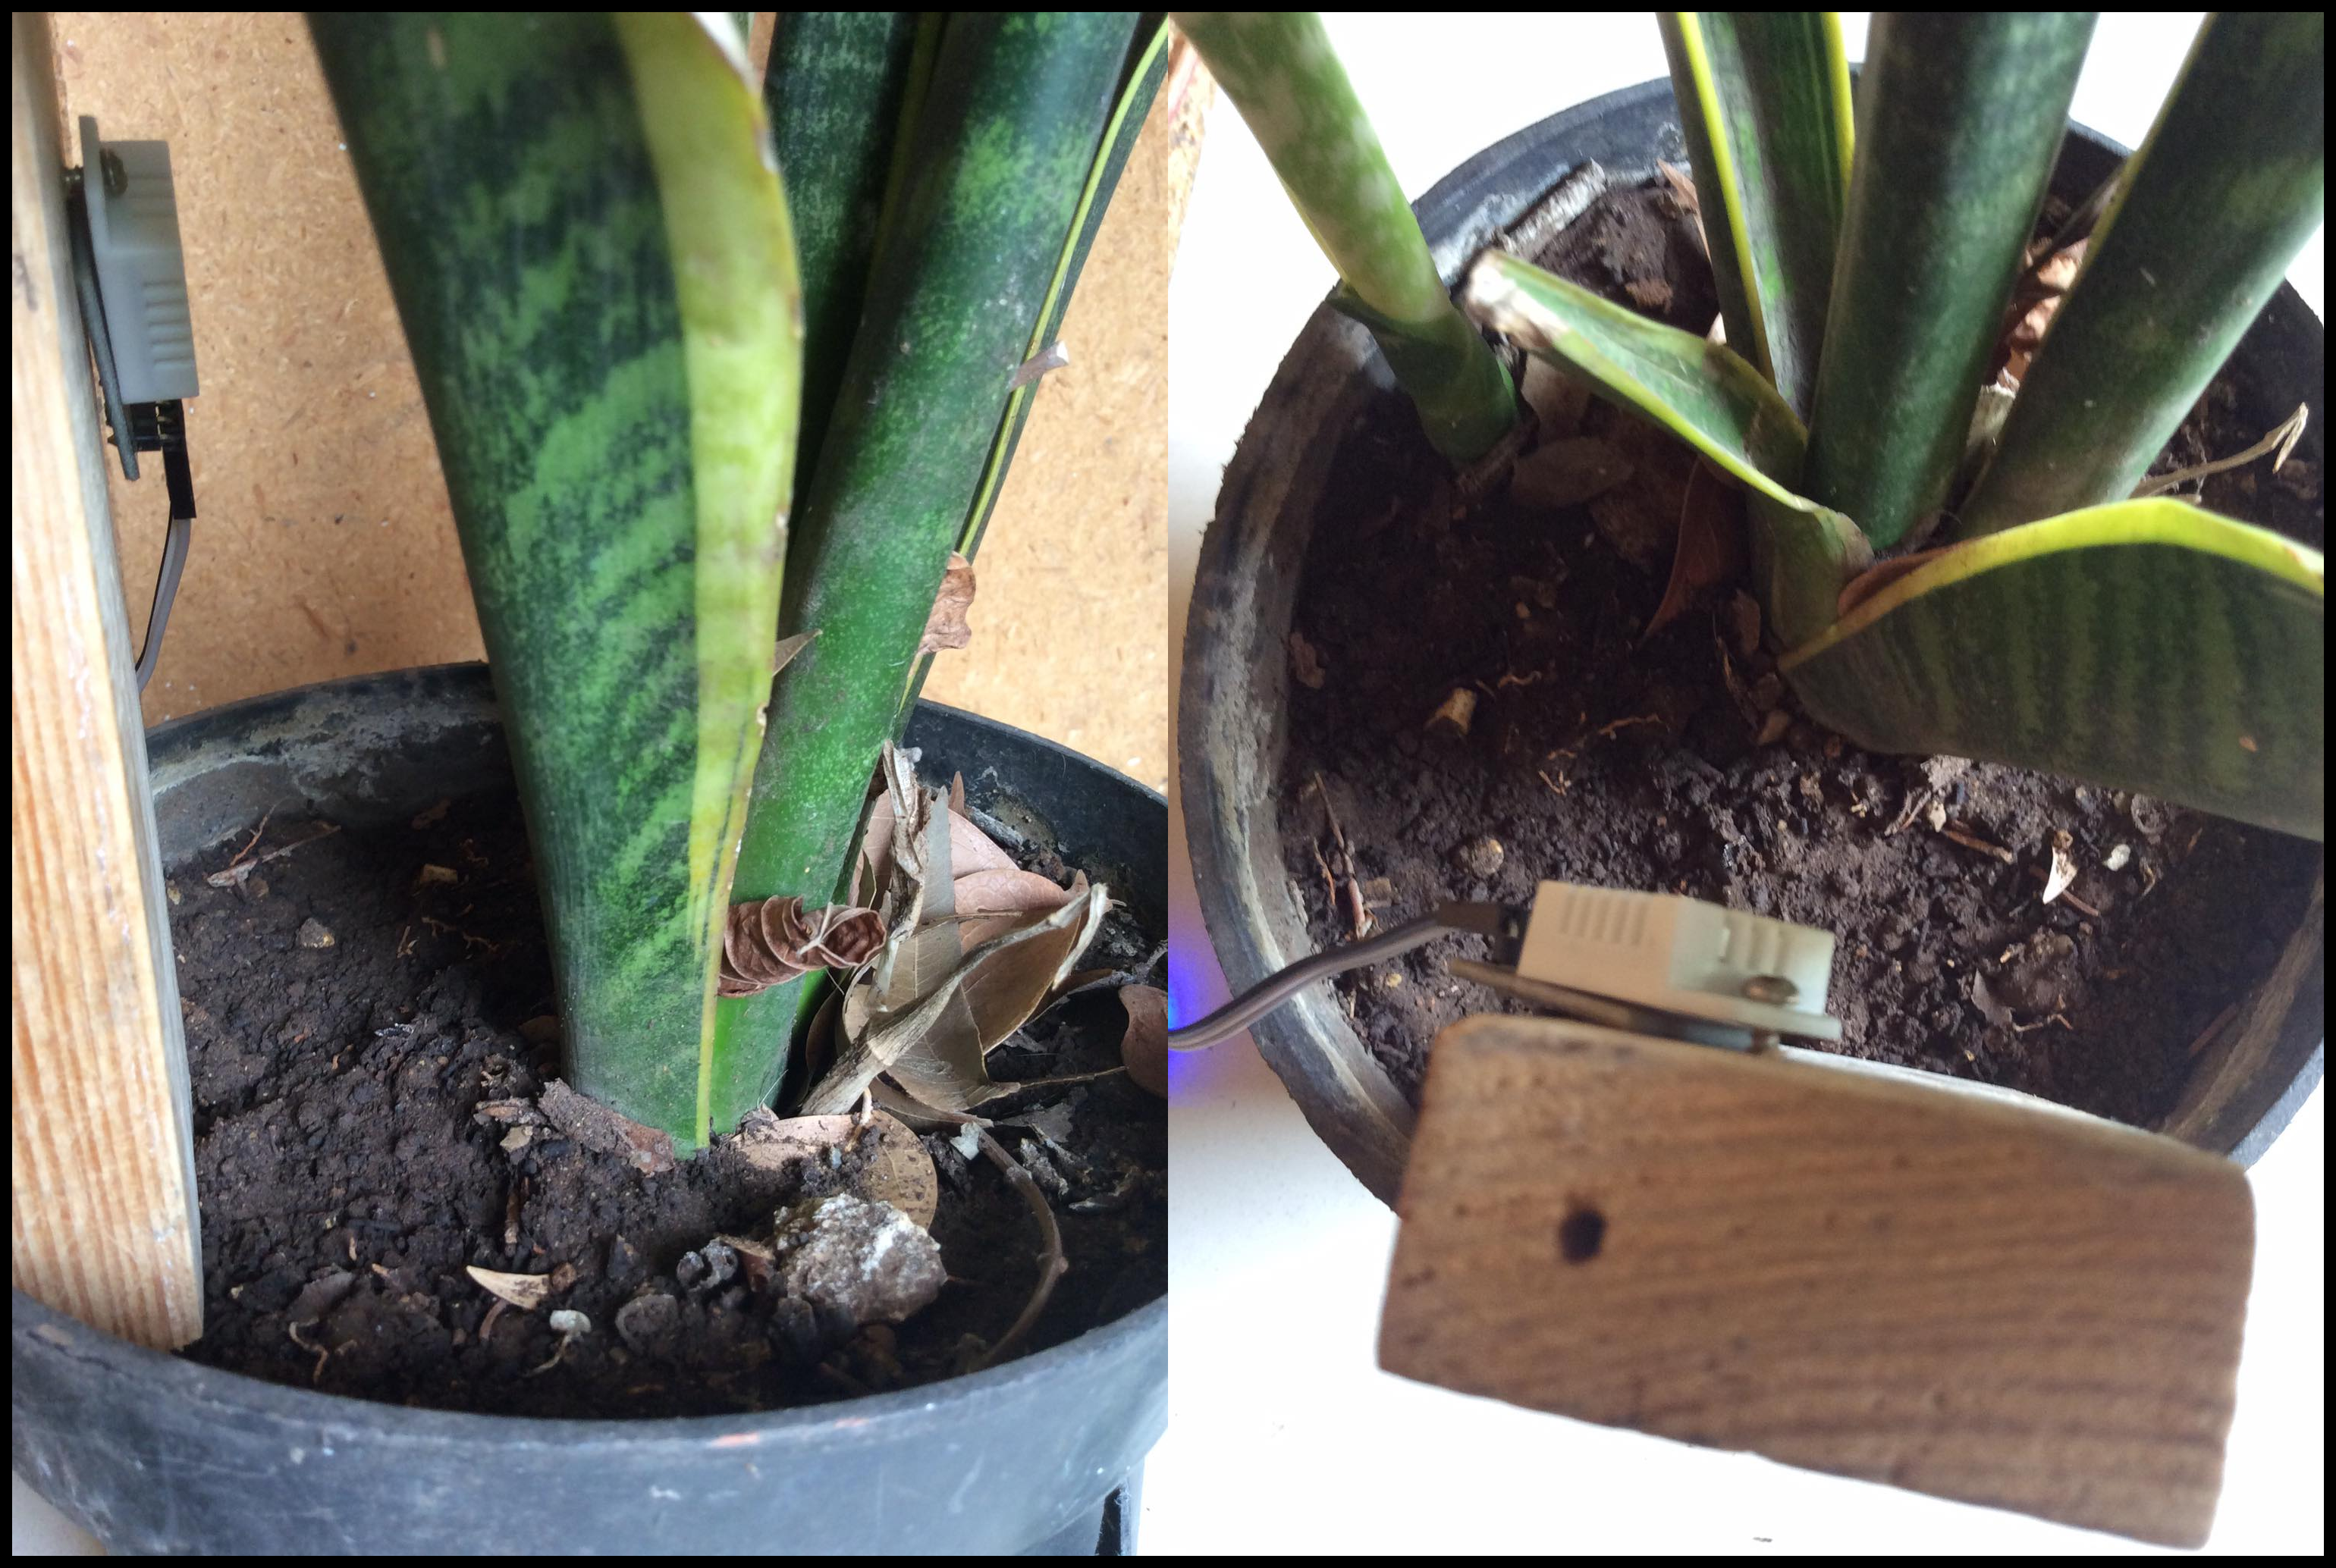
\includegraphics[width=0.48\textwidth]{2021_IoT_JoseRamon/figs/image.png}\\
          \end{tabular}
\end{center}
\end{column} 
\end{columns} 
\end{frame}



\begin{frame}{\citetitle{MarcoNuno_Revista_2021_10_00} (3)}
\begin{columns}
\begin{column}{0.40\textwidth}
La aplicación movil desarrollada tiene las siguientes funcionalidades:
\begin{itemize}
        \item Permite configurar los datos de conectividad con el Broker
        \item Establece parámetros de las alarmas y notificaciones
        \item Permite visualizar datos de manera gráfica
	\end{itemize}
\end{column}
\begin{column}{0.60\textwidth}  
\begin{center}
     \begin{tabular}{c}
         \includegraphics[width=0.32\textwidth]{2021_IoT_JoseRamon/figs/pantalla de configuracion.png}
\includegraphics[width=0.32\textwidth]{2021_IoT_JoseRamon/figs/pantalla de humedad.png}
\includegraphics[width=0.32\textwidth]{2021_IoT_JoseRamon/figs/pantalla de temperatura.png}\\

          \end{tabular}
\end{center}
\end{column} 
\end{columns} 
\end{frame}



\begin{frame}{\citetitle{MarcoNuno_Revista_2021_10_00} (4)}
\begin{columns}
\begin{column}{0.40\textwidth}
\begin{itemize}
        \item Una vez que la aplicación ha sido configurada, dependiendo de los umbrales establecidos, se emite una notificación al usuario cuando se rebazan dichos umbrales
        \item Esto permite detectar problemas y/o tomar acciones correctivas
	\end{itemize}
\end{column}
\begin{column}{0.60\textwidth}  
\begin{center}
     \begin{tabular}{c}
\includegraphics[width=0.48\textwidth]{2021_IoT_JoseRamon/figs/Alerta humedad.png}
\includegraphics[width=0.48\textwidth]{2021_IoT_JoseRamon/figs/Alerta Temperatura.png}\\
          \end{tabular}
\end{center}
\end{column} 
\end{columns} 
\end{frame}






